Since
\begin{align}
\vec{A} - \vec{B} &= \myvec{-2\\0\\0}\\
\vec{C} -\vec{B} &= \myvec{0\\-1\\0}
\end{align}
area of the rectangle is
\begin{align}
 \norm{\brak{\vec{A} -\vec{B}} \times \brak{\vec{C}-\vec{D}}}
= 2
\end{align} 
\iffalse
See Fig. 
   \ref{fig:chapters/12/10/4/12Rect_ABCD}
\begin{figure}[H]
  \centering
   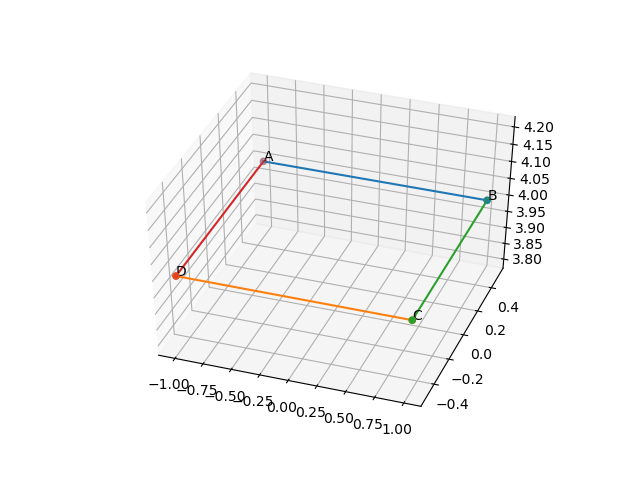
\includegraphics[width=0.75\columnwidth]{chapters/12/10/4/12/figs/Figure_1.png}
   \caption{}
   \label{fig:chapters/12/10/4/12Rect_ABCD}
\end{figure}
\fi




